\documentclass[11pt]{article}
\usepackage[a4paper, margin=1in]{geometry}
\usepackage[T1]{fontenc}
\usepackage{amsmath}
\usepackage{graphicx}
\graphicspath{{assets/}{./assets/}}
\usepackage{hyperref}
\usepackage{listings}
\usepackage{tikz}
\usepackage{tocloft}
\usepackage{xcolor}
\usepackage{enumitem}
\usepackage{microtype}
\usepackage[sc]{mathpazo} % Elegant body font
\usepackage{inconsolata}  % Nicer monospace for code
\usepackage{parskip}      % Space between paragraphs
\usepackage{fancyhdr}     % Header/footer
\usepackage{booktabs}     % Beautiful tables
\usepackage{longtable}    % Multi-page tables
\usepackage{array}
\usepackage{multirow}

% Brand and colors
\definecolor{BrandBlue}{HTML}{1E77D3}
\definecolor{BrandDark}{HTML}{0F2030}
\definecolor{BrandLight}{HTML}{F2F7FC}
\definecolor{AccentGreen}{HTML}{2ECC71}
\definecolor{AccentOrange}{HTML}{F39C12}

\hypersetup{
    colorlinks=true,
    linkcolor=BrandBlue,
    filecolor=magenta,
    urlcolor=BrandBlue,
    citecolor=BrandBlue
}

\usetikzlibrary{shapes.geometric, arrows, positioning, fit, calc}

\definecolor{codegreen}{rgb}{0,0.6,0}
\definecolor{codegray}{rgb}{0.5,0.5,0.5}
\definecolor{codepurple}{rgb}{0.58,0,0.82}
\definecolor{backcolour}{rgb}{0.97,0.98,1}

\lstdefinestyle{mystyle}{
    backgroundcolor=\color{backcolour},   
    commentstyle=\color{codegreen},
    keywordstyle=\color{BrandBlue},
    numberstyle=\tiny\color{codegray},
    stringstyle=\color{codepurple},
    basicstyle=\linespread{1.05}\ttfamily\footnotesize,
    breakatwhitespace=false,         
    breaklines=true,                 
    captionpos=b,                    
    keepspaces=true,                 
    numbers=left,                    
    numbersep=5pt,                  
    showspaces=false,                
    showstringspaces=false,
    showtabs=false,                  
    tabsize=2
}
\lstset{style=mystyle}

% Lists and spacing
\setlist[itemize]{leftmargin=1.2em}
\setlist[enumerate]{leftmargin=1.5em}

% Header and footer
\pagestyle{fancy}
\fancyhf{}
\fancyhead[L]{\textcolor{BrandDark}{\textbf{StudyFlow}}}
\fancyhead[R]{\textcolor{BrandBlue}{Technical Design}}
\fancyfoot[L]{\textcolor{BrandDark}{v1.0}}
\fancyfoot[R]{\thepage}

% TikZ setup
    ikzset{
        data/.style={draw, rounded corners, fill=BrandLight, minimum height=1.2em},
        process/.style={draw, rectangle, rounded corners=2pt, fill=white, minimum height=1.6em},
    store/.style={draw, cylinder, shape border rotate=90, aspect=0.25, fill=BrandLight},
    actor/.style={draw, circle, minimum size=1.3em}
}

% Handy macro
\newcommand{\product}{StudyFlow}

    itle{
    \vspace{1.5cm}
    {\Huge \textbf{\textcolor{BrandDark}{StudyFlow}}}\\[0.4em]
    {\Large \textcolor{BrandBlue}{Smart Academic Planner}}\\[0.8em]
    {\large Technical Design and Specification}
}
\author{Project Analysis by GitHub Copilot}
\date{\today}

\begin{document}

\maketitle
\thispagestyle{empty}
\vspace{-0.8em}
\begin{center}
\begin{minipage}{0.92\linewidth}
\begin{flushleft}
    extbf{Abstract}\\
\small {\product} is a client-first, data-informed academic planner that unifies course, assignment, and task management with proactive reminders and analytics. This document presents a detailed problem framing, user stories, architecture and design, a forward-looking API and deployment model, a quality and test strategy, and reference diagrams (DFD, ERD, UML). It also outlines security, performance, accessibility, and privacy considerations suitable for scaling from a single-device experience to a multi-tenant web service.
\end{flushleft}
\end{minipage}
\end{center}
\newpage

\tableofcontents
\newpage

\section*{Executive Summary}
\addcontentsline{toc}{section}{Executive Summary}
\begin{itemize}
    \item \textbf{Audience}: Students who need a unified planner; educators evaluating tooling; developers extending a modular SPA.
    \item \textbf{Core Value}: Consolidates deadlines across courses, prioritizes work, and surfaces insights to improve outcomes.
    \item \textbf{Now vs. Next}: Today, state and analytics are computed client-side using \texttt{localStorage}. Next, we introduce secure auth, a REST/GraphQL API, and push-based reminders for cross-device sync.
\end{itemize}

\section{Problem Statement}

In the contemporary academic landscape, students are inundated with a high volume of tasks, assignments, and deadlines across multiple courses. This complexity often leads to increased cognitive load, inefficient time management, and a reactive rather than proactive approach to learning. The absence of an integrated, intelligent system for tracking academic progress results in missed deadlines, last-minute stress, and a lack of insight into personal productivity patterns.

StudyFlow is engineered to address these challenges by providing a centralized, data-driven platform for academic task management. It aims to be more than a simple to-do list; it is a smart planner that leverages data analytics to offer actionable insights, proactive reminders, and a holistic view of a student's academic life. The core problem is the fragmentation of academic information and the lack of intelligent tools to synthesize this information into a personalized, optimized workflow. StudyFlow bridges this gap by offering a unified ecosystem for managing courses, assignments, and tasks, thereby empowering students to take control of their learning journey.

\section{User Stories}

The system is designed around the primary actor, the "Student," with a secondary "Guest" role for trial purposes.

\begin{itemize}
    \item \textbf{As a Student, I want to create a secure account and log in,} so that my academic data is private and persistent across sessions.
    \item \textbf{As a Student, I want to add, edit, and delete my courses for the semester,} so that I can organize my academic responsibilities by subject.
    \item \textbf{As a Student, I want to add assignments with titles, descriptions, due dates, and priority levels,} so that I can track all my graded work in one place.
    \item \textbf{As a Student, I want to create general tasks with due dates and priorities,} so that I can manage non-assignment related activities like "Review lecture notes" or "Prepare for exam."
    \item \textbf{As a Student, I want to see a consolidated dashboard,} so that I can get an immediate overview of my active courses, pending tasks, and high-priority items.
    \item \textbf{As a Student, I want to view upcoming deadlines on my dashboard,} so that I can prioritize my work effectively.
    \item \textbf{As a Student, I want to receive automated reminders for tasks and assignments that are due soon or overdue,} so that I can stay on top of my deadlines.
    \item \textbf{As a Student, I want to view an analytics dashboard,} so that I can understand my productivity patterns, such as my task completion rate and performance in different courses.
    \item \textbf{As a Guest User, I want to quickly access the app with sample data without creating an account,} so that I can evaluate its features before committing to registration.
\end{itemize}

\section{System Architecture and System Design}

While the current implementation is a client-side application, the architecture is designed with a forward-looking, scalable, server-based model in mind. The design follows a modular, service-oriented pattern.

\subsection{Architectural Model: Client-Server with Micro-frontend Influence}

The system is architected as a \textbf{Single Page Application (SPA)} that communicates with a conceptual backend via a RESTful API. The frontend itself is modular, with distinct components for Authentication, Data Management, and UI Rendering, mimicking a micro-frontend approach for maintainability.

\begin{itemize}
    \item \textbf{Client (Browser)}: The client is responsible for all UI rendering and state management. It is built with HTML5, CSS3, and modern JavaScript (ES6+). The client-side logic is partitioned into:
    \begin{itemize}
        \item \textbf{Auth Service (`auth.js`)}: Manages user sessions, registration, and login. In the current model, it interfaces with `localStorage` as a mock database.
        \item \textbf{Data Service (`app.js`)}: The `DataManager` class acts as an Object-Relational Mapping (ORM) layer, abstracting the data persistence logic (currently `localStorage`). It provides a clean API for CRUD operations on courses, assignments, and tasks.
        \item \textbf{Analytics Service (`analytics.js`)}: A client-side data processing engine that computes and visualizes metrics from the data service.
        \item \textbf{View Components (`app.js`, `index.html`)}: A set of functions responsible for rendering the dynamic HTML for each section (Dashboard, Courses, etc.).
    \end{itemize}
    \item \textbf{Conceptual Backend Server}: A stateless server that would expose a REST API for the client.
    \begin{itemize}
        \item \textbf{Authentication Endpoint}: Handles user registration and JWT (JSON Web Token) generation.
        \item \textbf{API Gateway}: A single entry point for all client requests, routing them to the appropriate microservices.
        \item \textbf{Data Service}: A microservice responsible for all business logic related to courses, tasks, and assignments.
        \item \textbf{Notification Service}: A service to manage and push real-time reminders (e.g., via WebSockets or Push API).
    \end{itemize}
    \item \textbf{Database}: A NoSQL database like MongoDB would be ideal for storing user data due to its flexible schema, which aligns well with the structure of courses, tasks, and assignments.
\end{itemize}

\subsection{Data Model}
The core data entities are Users, Courses, Assignments, and Tasks.

\begin{itemize}
    \item \textbf{User}: \{ `id`, `username`, `email`, `passwordHash`, `createdAt` \}
    \item \textbf{Course}: \{ `id`, `userId`, `name`, `code`, `instructor`, `color`, `createdAt` \}
    \item \textbf{Assignment}: \{ `id`, `userId`, `courseId`, `title`, `description`, `dueDate`, `priority`, `completed`, `createdAt` \}
    \item \textbf{Task}: \{ `id`, `userId`, `courseId` (optional), `title`, `description`, `dueDate`, `priority`, `completed`, `completedAt`, `createdAt` \}
\end{itemize}

\subsection{Technology Stack}
\begin{center}
\begin{tabular}{@{}p{0.28\linewidth} p{0.66\linewidth}@{}}
	oprule
	extbf{Layer} & \textbf{Technology} \\
\midrule
UI/SPA & HTML5, CSS3, Vanilla ES6+ (modular services); optional Tailwind/Bootstrap for scale \\
State \& Storage (current) & Web Storage API (\texttt{localStorage}) per-user keyspace \\
Visualization & SVG-based custom charts (no heavy deps) \\
Auth (future) & OAuth2.1 / OIDC with PKCE, JWT access tokens, refresh token rotation \\
API (future) & REST/JSON or GraphQL over HTTPS; rate-limited behind API Gateway \\
Database (future) & MongoDB (flexible schema, TTL indexes for reminders) \\
Async (future) & Message queue (e.g., RabbitMQ) for reminder fan-out and email/push workers \\
\bottomrule
\end{tabular}
\end{center}

\subsection{Key Quality Attributes}
\begin{itemize}
    \item \textbf{Reliability}: Idempotent APIs, deterministic analytics, and safe writes with server-side validation.
    \item \textbf{Performance}: Incremental rendering; O(1) access patterns for hot lists; lazy-loading archives.
    \item \textbf{Security}: Strong hashing (Argon2id/bcrypt), token hardening (DPoP/MTLS optional), strict content security policy.
    \item \textbf{Accessibility}: WCAG~2.1 AA contrast, keyboard-first flows, ARIA roles on dynamic widgets.
\end{itemize}

\subsection{Component Diagram}
\begin{figure}[h!]
\centering
\begin{tikzpicture}[node distance=1.6cm]
    \node[process, minimum width=3.2cm] (auth) {Auth Service\\\small (\texttt{auth.js})};
    \node[process, right=2.4cm of auth, minimum width=3.6cm] (data) {Data Service\\\small (\texttt{DataManager})};
    \node[process, below=1.6cm of data, minimum width=3.6cm] (analytics) {Analytics\\\small (charts \& insights)};
    \node[process, below=1.6cm of auth, minimum width=3.2cm] (ui) {Views\\\small (Dashboard/Courses/...)};
    \node[store, right=2.4cm of data, minimum width=1.8cm, minimum height=1.8cm] (storage) {localStorage};

    \draw[->, thick] (ui) -- node[above] {login/logout} (auth);
    \draw[->, thick] (ui) -- node[above] {CRUD ops} (data);
    \draw[->, thick] (data) -- node[above] {persist} (storage);
    \draw[->, thick] (data) -- node[right] {datasets} (analytics);
    \draw[->, thick] (analytics) -- node[left] {widgets} (ui);
\end{tikzpicture}
\caption{Frontend component interactions (current client-only model)}
\end{figure}

% Image: Architecture Overview (provided as arc.png)
\begin{figure}[h!]
\centering
\includegraphics[width=0.95\linewidth]{arc.png}
\caption{High-level architecture overview: client SPA today, with future API, services, and data stores.}
\end{figure}

\subsection{Representative Sequence (Add Task)}
\begin{figure}[h!]
\centering
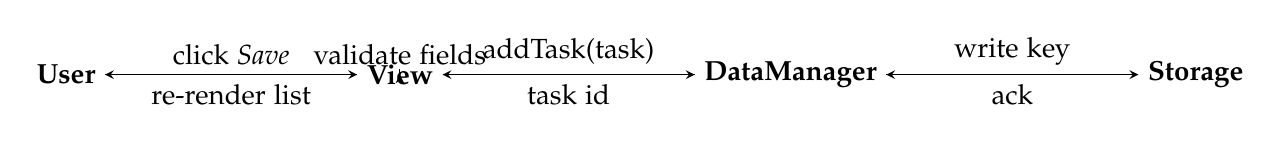
\begin{tikzpicture}[>=stealth, node distance=2.2cm]
    \node (u)  {\textbf{User}};
    \node[right=3.2cm of u] (v) {\textbf{View}};
    \node[right=3.2cm of v] (d) {\textbf{DataManager}};
    \node[right=3.2cm of d] (s) {\textbf{Storage}};
    \draw[->] (u) -- node[above]{click \emph{Save}} (v);
    \draw[->] (v) -- node[above]{validate fields} (v);
    \draw[->] (v) -- node[above]{addTask(task)} (d);
    \draw[->] (d) -- node[above]{write key} (s);
    \draw[->] (s) -- node[below]{ack} (d);
    \draw[->] (d) -- node[below]{task id} (v);
    \draw[->] (v) -- node[below]{re-render list} (u);
\end{tikzpicture}
\caption{Happy-path sequence for adding a task}
\end{figure}

\subsection{Security and Privacy}
\begin{itemize}
    \item \textbf{Authentication}: Transition to OIDC with short-lived access tokens and rotating refresh tokens; device binding where feasible.
    \item \textbf{Password storage}: Use Argon2id with memory-hard parameters; enforce strong password policy and have breach checking (k-Anonymity).
    \item \textbf{Transport}: Enforce TLS~1.3; HSTS; same-site cookies (\texttt{Strict}); CSRF tokens on state-changing requests.
    \item \textbf{Privacy}: Data minimization, user export/delete (GDPR Art.~15/17), regional data residency options.
\end{itemize}

\subsection{Performance and Scalability}
\begin{itemize}
    \item \textbf{Client}: Batch DOM updates, memoize computed aggregates, virtualize long lists.
    \item \textbf{Server (future)}: Use CQRS for analytics vs. writes; cache hot queries (e.g., next 7 days) with TTL.
    \item \textbf{Reminders}: Pre-compute next trigger per item; wheel-timer buckets to scale to millions of schedules.
\end{itemize}

\subsection{Deployment Overview (Future)}
\begin{figure}[h!]
\centering
\begin{tikzpicture}[node distance=1.6cm]
    \node[process, minimum width=3.2cm] (client) {SPA Client};
    \node[process, right=1.8cm of client, minimum width=2.8cm] (cdn) {CDN};
    \node[process, right=1.8cm of cdn, minimum width=3.2cm] (api) {API Gateway};
    \node[process, below=1.2cm of api, minimum width=3.2cm] (svc) {Domain Services};
    \node[store, right=2.0cm of svc, minimum width=1.8cm, minimum height=1.8cm] (db) {MongoDB};
    \node[store, below=1.2cm of db, minimum width=1.6cm, minimum height=1.6cm] (cache) {Redis};
    \node[process, below=1.2cm of svc, minimum width=3.2cm] (notify) {Reminder Workers};

    \draw[->, thick] (client) -- node[above]{HTTPS} (cdn);
    \draw[->, thick] (cdn) -- node[above]{/api/*} (api);
    \draw[->, thick] (api) -- node[right]{RPC/REST} (svc);
    \draw[->, thick] (svc) -- node[above]{read/write} (db);
    \draw[->, thick] (svc) -- node[right]{cache} (cache);
    \draw[->, thick] (notify) -- node[right]{queries} (db);
    \draw[->, thick] (notify) -- node[left]{events} (api);
\end{tikzpicture}
\caption{Future deployment topology for a multi-service backend with caching and workers.}
\end{figure}

\section{Design of Tests}

A comprehensive testing strategy would involve unit, integration, and end-to-end (E2E) tests.

\subsection{Unit Testing}
Unit tests would focus on isolating and verifying the smallest parts of the application.
\begin{itemize}
    \item \textbf{`auth.js`}:
        \begin{itemize}
            \item Test email validation with valid and invalid inputs.
            \item Test password length and match constraints.
            \item Mock `localStorage` to test user registration (checking for duplicates) and login (password verification).
        \end{itemize}
    \item \textbf{`app.js` (`DataManager`)}:
        \begin{itemize}
            \item Mock `localStorage` to test all CRUD operations: `addCourse`, `updateCourse`, `deleteCourse`, etc.
            \item Verify that IDs and timestamps are correctly generated on creation.
            \item Test `toggleTaskCompletion` to ensure the `completed` and `completedAt` fields are updated correctly.
        \end{itemize}
    \item \textbf{`analytics.js`}:
        \begin{itemize}
            \item Create mock data sets to test the calculation logic for `renderCompletionRate`, `renderPriorityChart`, `renderWeeklyProgress`, and `renderCoursePerformance`.
            \item Test edge cases, such as when there are no tasks or courses.
        \end{itemize}
\end{itemize}

\subsection{Integration Testing}
Integration tests would verify that different modules work together as expected.
\begin{itemize}
    \item \textbf{Auth and Data}: Test that after a user logs in, the `DataManager` is initialized with the correct `userId` and loads the correct data.
    \item \textbf{Data and UI}: Test that after adding a new course via the UI, the course list view is correctly re-rendered with the new data.
    \item \textbf{Reminders and Data}: Test that the `checkReminders` function correctly identifies upcoming tasks from the `DataManager` and triggers a notification.
\end{itemize}

\subsection{End-to-End (E2E) Testing}
E2E tests would simulate real user workflows from start to finish using a framework like Cypress or Playwright.
\begin{itemize}
    \item \textbf{Full User Journey}:
        \begin{enumerate}
            \item A user registers for a new account.
            \item The user logs in.
            \item The user creates a new course.
            \item The user adds an assignment to that course.
            \item The user creates a standalone task.
            \item The user marks the task as complete.
            \item The user navigates to the analytics page and verifies the completion rate has updated.
            \item The user logs out.
        \end{enumerate}
\end{itemize}

\subsection{Regression Testing}
Regression testing ensures that new code changes do not break existing functionality. This is critical for maintaining system stability as features are added or refactored.

\subsubsection{Strategy}
\begin{itemize}
    \item \textbf{Automated Test Suite}: Maintain a comprehensive suite of unit, integration, and E2E tests that are executed on every code commit via CI/CD pipeline (GitHub Actions, GitLab CI, or Jenkins).
    \item \textbf{Test Coverage Targets}: Aim for $\geq 80\%$ code coverage for critical paths (auth, data persistence, CRUD operations) and $\geq 60\%$ overall coverage.
    \item \textbf{Baseline Test Set}: Define a core set of regression tests covering:
        \begin{itemize}
            \item User authentication and session management
            \item All CRUD operations for courses, assignments, and tasks
            \item Data persistence and retrieval across sessions
            \item Dashboard rendering and data aggregation
            \item Analytics calculations and chart rendering
            \item Reminder generation and notification triggering
        \end{itemize}
\end{itemize}

\subsubsection{Regression Test Scenarios}
\begin{itemize}
    \item \textbf{Data Integrity}: After refactoring the `DataManager` class, verify that all existing data operations (add, update, delete, query) produce identical results.
    \item \textbf{UI Consistency}: When CSS or HTML structure changes, verify that all views render correctly and interactive elements remain functional.
    \item \textbf{API Contract (Future)}: When backend APIs evolve, ensure backward compatibility or proper versioning; mock old API responses to test client resilience.
    \item \textbf{Cross-Browser Compatibility}: Run regression tests across Chrome, Firefox, Safari, and Edge to catch browser-specific issues.
    \item \textbf{Performance Baselines}: Track execution time of key operations (login, data load, analytics rendering) to detect performance regressions.
\end{itemize}

\subsubsection{Regression Testing Tools}
\begin{center}
\begin{tabular}{@{}p{0.28\linewidth} p{0.66\linewidth}@{}}
\toprule
\textbf{Tool} & \textbf{Purpose} \\
\midrule
Jest / Mocha & Unit and integration test automation with snapshot testing \\
Cypress / Playwright & E2E regression tests with visual regression capabilities \\
Percy / Chromatic & Visual regression testing for UI consistency \\
Istanbul / NYC & Code coverage reporting to identify untested paths \\
Lighthouse CI & Performance regression tracking (load time, bundle size) \\
\bottomrule
\end{tabular}
\end{center}

\subsection{Mutation Testing}
Mutation testing evaluates the quality and effectiveness of the test suite by introducing small, deliberate faults (mutations) into the code and checking if tests catch them.

\subsubsection{Mutation Testing Concepts}
\begin{itemize}
    \item \textbf{Mutant}: A modified version of the code with a single syntactic change (e.g., changing \texttt{+} to \texttt{-}, \texttt{===} to \texttt{!==}, removing a condition).
    \item \textbf{Killed Mutant}: A mutant that causes at least one test to fail, indicating the test suite detected the fault.
    \item \textbf{Survived Mutant}: A mutant that passes all tests, revealing a gap in test coverage or weak assertions.
    \item \textbf{Mutation Score}: Percentage of mutants killed by tests: $\text{Score} = \frac{\text{Killed Mutants}}{\text{Total Mutants}} \times 100\%$. Target: $\geq 75\%$.
\end{itemize}

\subsubsection{Mutation Operators for StudyFlow}
\begin{center}
\begin{tabular}{@{}p{0.28\linewidth} p{0.66\linewidth}@{}}
\toprule
\textbf{Operator} & \textbf{Example Mutation} \\
\midrule
Arithmetic & Change \texttt{count + 1} to \texttt{count - 1} \\
Relational & Change \texttt{dueDate < today} to \texttt{dueDate <= today} \\
Logical & Change \texttt{\&\&} to \texttt{||} in conditionals \\
Negation & Change \texttt{task.completed} to \texttt{!task.completed} \\
Statement Deletion & Remove \texttt{this.save('tasks', this.tasks)} \\
Constant Replacement & Change \texttt{priority === 'high'} to \texttt{priority === 'low'} \\
Return Value & Change \texttt{return true} to \texttt{return false} \\
\bottomrule
\end{tabular}
\end{center}

\subsubsection{Mutation Testing Scenarios for StudyFlow}
\begin{itemize}
    \item \textbf{Authentication Logic}:
        \begin{itemize}
            \item Mutate password comparison from \texttt{===} to \texttt{!==}; tests should fail.
            \item Remove email format validation; tests should catch invalid registrations.
        \end{itemize}
    \item \textbf{Data Persistence}:
        \begin{itemize}
            \item Remove the \texttt{save()} call after adding a task; tests should verify persistence.
            \item Mutate the key used in \texttt{localStorage.getItem}; tests should detect data retrieval failure.
        \end{itemize}
    \item \textbf{Task Completion}:
        \begin{itemize}
            \item Change \texttt{task.completed = true} to \texttt{task.completed = false}; tests should verify completion state.
            \item Remove \texttt{completedAt} timestamp assignment; tests should check timestamp presence.
        \end{itemize}
    \item \textbf{Analytics Calculations}:
        \begin{itemize}
            \item Mutate completion rate formula from \texttt{completed / total} to \texttt{completed / (total + 1)}; tests should verify exact percentages.
            \item Change priority filter from \texttt{=== 'high'} to \texttt{!== 'high'}; tests should detect incorrect counts.
        \end{itemize}
    \item \textbf{Reminder Logic}:
        \begin{itemize}
            \item Mutate the 24-hour threshold from \texttt{<= 24} to \texttt{< 24}; boundary tests should fail.
            \item Remove the overdue check; tests should verify overdue items are flagged.
        \end{itemize}
\end{itemize}

\subsubsection{Mutation Testing Tools and Workflow}
\begin{center}
\begin{tabular}{@{}p{0.28\linewidth} p{0.66\linewidth}@{}}
\toprule
\textbf{Tool} & \textbf{Description} \\
\midrule
Stryker (JavaScript) & Industry-standard mutation testing framework for JS/TS; integrates with Jest, Mocha \\
Mutmut (Python) & For future Python-based services or analytics scripts \\
PIT (Java) & If migrating to Java-based backend services \\
\bottomrule
\end{tabular}
\end{center}

\textbf{Workflow:}
\begin{enumerate}
    \item Run mutation testing tool (e.g., \texttt{npx stryker run}) to generate mutants.
    \item Tool executes test suite against each mutant and reports killed vs. survived.
    \item Analyze survived mutants to identify:
        \begin{itemize}
            \item Missing test cases
            \item Weak assertions (e.g., checking only presence, not value)
            \item Equivalent mutants (semantically identical code that should be marked)
        \end{itemize}
    \item Enhance tests to kill survived mutants, aiming for $\geq 75\%$ mutation score.
    \item Integrate mutation testing into CI pipeline (weekly or on major releases due to execution cost).
\end{enumerate}

\subsubsection{Benefits and Limitations}
\textbf{Benefits:}
\begin{itemize}
    \item Reveals weaknesses in test assertions that traditional coverage metrics miss.
    \item Forces developers to write precise, meaningful tests.
    \item Increases confidence in the robustness of the test suite.
\end{itemize}

\textbf{Limitations:}
\begin{itemize}
    \item Computationally expensive; execution time scales with codebase size and mutant count.
    \item Equivalent mutants (mutations that don't change behavior) require manual review.
    \item High mutation scores don't guarantee absence of all bugs, only that tests are sensitive to common faults.
\end{itemize}

\subsection{Test Matrix (Representative)}
\begin{center}
\begin{longtable}{@{}p{0.22\linewidth} p{0.52\linewidth} p{0.18\linewidth}@{}}
	oprule
	extbf{Area} & \textbf{Key Cases} & \textbf{Priority} \\
\midrule\endhead
Auth & Register, login, bad password, existing user, email format & High \\
Courses & Add, edit, delete, list empty state, persistence & High \\
Assignments & CRUD, validation, due date parsing, course linkage & High \\
Tasks & CRUD, priority filter, toggle complete, sorting & High \\
Analytics & Zero-data, partial-data, completion %, weekly bars & Medium \\
Reminders & \(\leq 24\,\text{h}\), overdue, sort order, badge counts & High \\
Import/Export & Round-trip fidelity, schema mismatch, error handling & Medium \\
\bottomrule
\end{longtable}
\end{center}

\subsection{Edge Cases}
\begin{itemize}
    \item Tasks without due dates should not appear in urgency lists; ensure stable sorting.
    \item Mixed timezones across entries; normalize to ISO 8601 UTC for computation.
    \item Deleting a course with linked tasks/assignments prompts confirmation and preserves orphaned tasks or offers reassignment.
\end{itemize}

\newpage
\section{Appendix}

\subsection{SRS (Software Requirements Specification)}

\subsubsection{Functional Requirements}
\begin{itemize}
    \item \textbf{FR1: User Authentication}: The system shall allow users to register, log in, and log out.
    \item \textbf{FR2: Course Management}: The system shall allow users to perform CRUD (Create, Read, Update, Delete) operations on courses.
    \item \textbf{FR3: Assignment Management}: The system shall allow users to perform CRUD operations on assignments, which must be linked to a course.
    \item \textbf{FR4: Task Management}: The system shall allow users to perform CRUD operations on tasks. Tasks can optionally be linked to a course.
    \item \textbf{FR5: Dashboard}: The system shall display a dashboard summarizing key metrics (e.g., total courses, pending tasks).
    \item \textbf{FR6: Analytics}: The system shall provide visualizations for task completion rates, priority distribution, and weekly progress.
    \item \textbf{FR7: Reminders}: The system shall automatically check for and notify the user of impending deadlines.
\end{itemize}

\subsubsection{Non-Functional Requirements}
\begin{itemize}
    \item \textbf{NFR1: Performance}: The UI must load in under 3 seconds. UI updates in response to user actions must feel instantaneous ($<\,200$\,ms).
    \item \textbf{NFR2: Usability}: The application must be intuitive and usable without a manual. It must be responsive and function on mobile, tablet, and desktop browsers.
    \item \textbf{NFR3: Security}: All user passwords must be hashed before storage. (Note: `btoa` is a placeholder for a proper hashing algorithm like Argon2 or bcrypt).
    \item \textbf{NFR4: Data Persistence}: All user-generated data must be saved and persist between sessions.
\end{itemize}

\subsubsection{API (Future) – Representative Endpoints}
\begin{tabular}{@{}p{0.16\linewidth} p{0.44\linewidth} p{0.32\linewidth}@{}}
	oprule
Method & Endpoint & Notes \\
\midrule
POST & /auth/register & Creates user, returns verification challenge \\
POST & /auth/login & Issues JWT (short-lived) + refresh token \\
GET & /courses & List user courses \\
POST & /courses & Create course \\
GET & /tasks?dueBefore=... & Query tasks by time window/priority \\
PATCH & /tasks/{id} & Partial update; ETag required \\
\bottomrule
\end{tabular}

\subsection{DFD (Data Flow Diagram)}

\begin{figure}[h!]
\centering
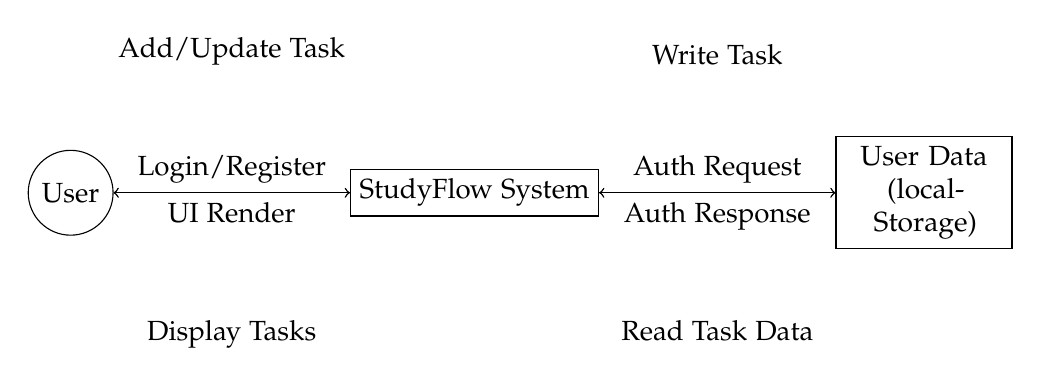
\begin{tikzpicture}[node distance=3cm, auto]
    % Nodes
    \node[draw, circle] (user) {User};
    \node[draw, rectangle, right=of user] (system) {StudyFlow System};
    \node[draw, rectangle, right=of system, text width=2cm, align=center] (datastore) {User Data (localStorage)};

    % Arrows
    \draw[->] (user) -- node[above] {Login/Register} (system);
    \draw[->] (system) -- node[above] {Auth Request} (datastore);
    \draw[->] (datastore) -- node[below] {Auth Response} (system);
    \draw[->] (system) -- node[below] {UI Render} (user);
    
    \draw[->] (user) -- node[above, yshift=1.5cm] {Add/Update Task} (system);
    \draw[->] (system) -- node[above, yshift=1.5cm] {Write Task} (datastore);
    \draw[->] (datastore) -- node[below, yshift=-1.5cm] {Read Task Data} (system);
    \draw[->] (system) -- node[below, yshift=-1.5cm] {Display Tasks} (user);
\end{tikzpicture}
\caption{Level 0 DFD for StudyFlow}
\end{figure}

\subsection{ERD (Entity-Relationship Diagram)}

\begin{figure}[h!]
\centering
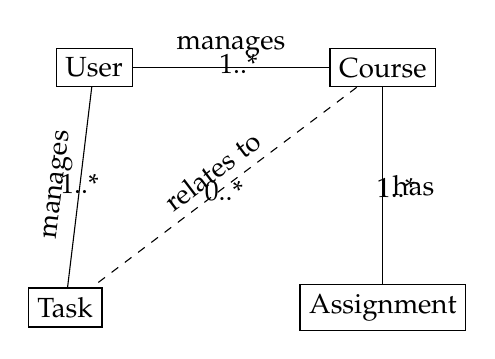
\begin{tikzpicture}[node distance=2.5cm, auto]
    % Entities
    \node[draw, rectangle] (user) {User};
    \node[draw, rectangle, right=of user] (course) {Course};
    \node[draw, rectangle, below=of course] (assignment) {Assignment};
    \node[draw, rectangle, left=of assignment] (task) {Task};

    % Relationships
    \draw[-] (user) -- node[above] {manages} (course);
    \draw[-] (user) -- node[above, sloped] {manages} (task);
    \draw[-] (course) -- node[right] {has} (assignment);
    \draw[dashed] (course) -- node[above, sloped] {relates to} (task);
    
    % Cardinality
    \node at ($(user)!0.5!(course)$) [above, yshift=-0.2cm] {1..*};
    \node at ($(user)!0.5!(task)$) [above, yshift=-0.2cm] {1..*};
    \node at ($(course)!0.5!(assignment)$) [right, xshift=-0.2cm] {1..*};
    \node at ($(course)!0.5!(task)$) [below, yshift=0.2cm] {0..*};
\end{tikzpicture}
\caption{Entity-Relationship Diagram for StudyFlow}
\end{figure}

\subsection{UML Diagrams}

\subsubsection{Use Case Diagram}
\begin{figure}[h!]
\centering
\begin{tikzpicture}
    \node[draw, ellipse] (uc1) at (0,0) {Manage Courses};
    \node[draw, ellipse] (uc2) at (0,-1.5) {Manage Assignments};
    \node[draw, ellipse] (uc3) at (0,-3) {Manage Tasks};
    \node[draw, ellipse] (uc4) at (4,0) {View Dashboard};
    \node[draw, ellipse] (uc5) at (4,-1.5) {View Analytics};
    \node[draw, ellipse] (uc6) at (4,-3) {Authenticate};
        % Simple actor glyph (no external image required)
        \node[actor] (actor) at (-4, -1.5) {};
        \node[below=0.1cm of actor] {Student};
        \draw[-] (actor) -- (uc1);
        \draw[-] (actor) -- (uc2);
        \draw[-] (actor) -- (uc3);
        \draw[-] (actor) -- (uc4);
        \draw[-] (actor) -- (uc5);
        \draw[-] (actor) -- (uc6);
\end{tikzpicture}
\caption{Use Case Diagram}
\end{figure}

\subsubsection{Class Diagram (from asset)}
\begin{figure}[h!]
\centering
\includegraphics[width=0.85\linewidth]{class.png}
\caption{UML Class Diagram (imported).}
\end{figure}

\subsubsection{Class Diagram (Simplified)}
\begin{figure}[h!]
\centering
\begin{tikzpicture}[node distance=2.2cm]
    \node[draw, rounded corners, align=left] (dm) {\textbf{DataManager}\\\hline
    	extit{- userId: string}\\
    	extit{- courses: Course[]}\\
    	extit{- assignments: Assignment[]}\\
    	extit{- tasks: Task[]}\\\hline
    + addCourse(c)\\
    + updateCourse(id, c)\\
    + addTask(t)\\
    + toggleTaskCompletion(id)\\};
\end{tikzpicture}
\caption{Core class sketch for client-side model}
\end{figure}

\subsubsection{Activity Diagram}
\begin{figure}[h!]
\centering
\includegraphics[width=0.9\linewidth]{activity.png}
\caption{Activity Diagram (imported) illustrating a typical task flow.}
\end{figure}

\subsubsection{Reminder Notification Sequence}
\begin{figure}[h!]
\centering
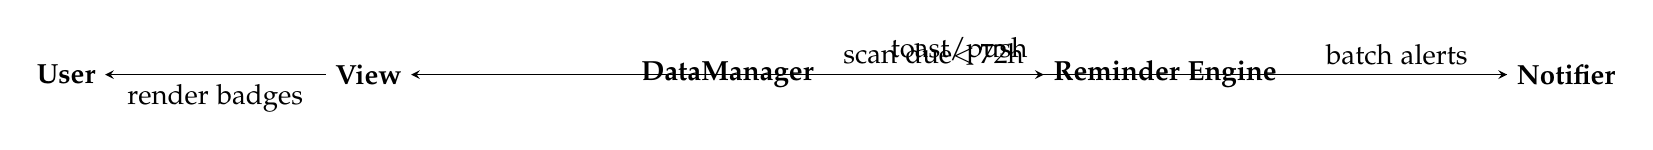
\begin{tikzpicture}[>=stealth, node distance=2.6cm]
    \node (u)  {\textbf{User}};
    \node[right=2.8cm of u] (v) {\textbf{View}};
    \node[right=2.8cm of v] (dm) {\textbf{DataManager}};
    \node[right=2.8cm of dm] (rem) {\textbf{Reminder Engine}};
    \node[right=2.8cm of rem] (not) {\textbf{Notifier}};
    \draw[->] (dm) -- node[above]{scan due\/$<$\,72h} (rem);
    \draw[->] (rem) -- node[above]{batch alerts} (not);
    \draw[->] (not) -- node[above]{toast/push} (v);
    \draw[->] (v) -- node[below]{render badges} (u);
\end{tikzpicture}
\caption{Sequence overview for deadline reminder surfacing.}
\end{figure}

\subsection{Code Listing / GitHub Link}

The project is a client-side application. The core logic for data management is encapsulated in the `DataManager` class in `app.js`.

\begin{lstlisting}[language=JavaScript, caption={DataManager Class from app.js}]
// Data Storage Manager
class DataManager {
    constructor(userId) {
        this.userId = userId;
        this.courses = this.load('courses') || [];
        this.assignments = this.load('assignments') || [];
        this.tasks = this.load('tasks') || [];
    }

    load(key) {
        const data = localStorage.getItem(`${this.userId}_${key}`);
        return data ? JSON.parse(data) : null;
    }

    save(key, data) {
        localStorage.setItem(`${this.userId}_${key}`, JSON.stringify(data));
    }

    // Courses
    getCourses() {
        return this.courses;
    }

    addCourse(course) {
        course.id = Date.now().toString();
        course.createdAt = new Date().toISOString();
        this.courses.push(course);
        this.save('courses', this.courses);
        return course;
    }
    
    // ... other CRUD methods for courses, assignments, and tasks
}
\end{lstlisting}

A public GitHub repository can be provided for full source code access:
\url{https://github.com/your-username/studyflow-planner}

\end{document}
